
\documentclass[10pt]{beamer}

\usepackage{algpseudocode}

\usetheme{Montpellier}
\usecolortheme{rose}

% page numbers, from
% https://tex.stackexchange.com/questions/137022/how-to-insert-page-number-in-beamer-navigation-symbols
\expandafter\def\expandafter\insertshorttitle\expandafter{%
  \insertshorttitle\hfill%
  \insertframenumber\,/\,\inserttotalframenumber}

\newcommand{\stanza}{ \\~\ }

\title{04. Randomization}
\subtitle{CPSC 535}
\author{Kevin A. Wortman}
\institute{ 
\includegraphics[height=2cm]{csuf-logo-cmyk} }
\date{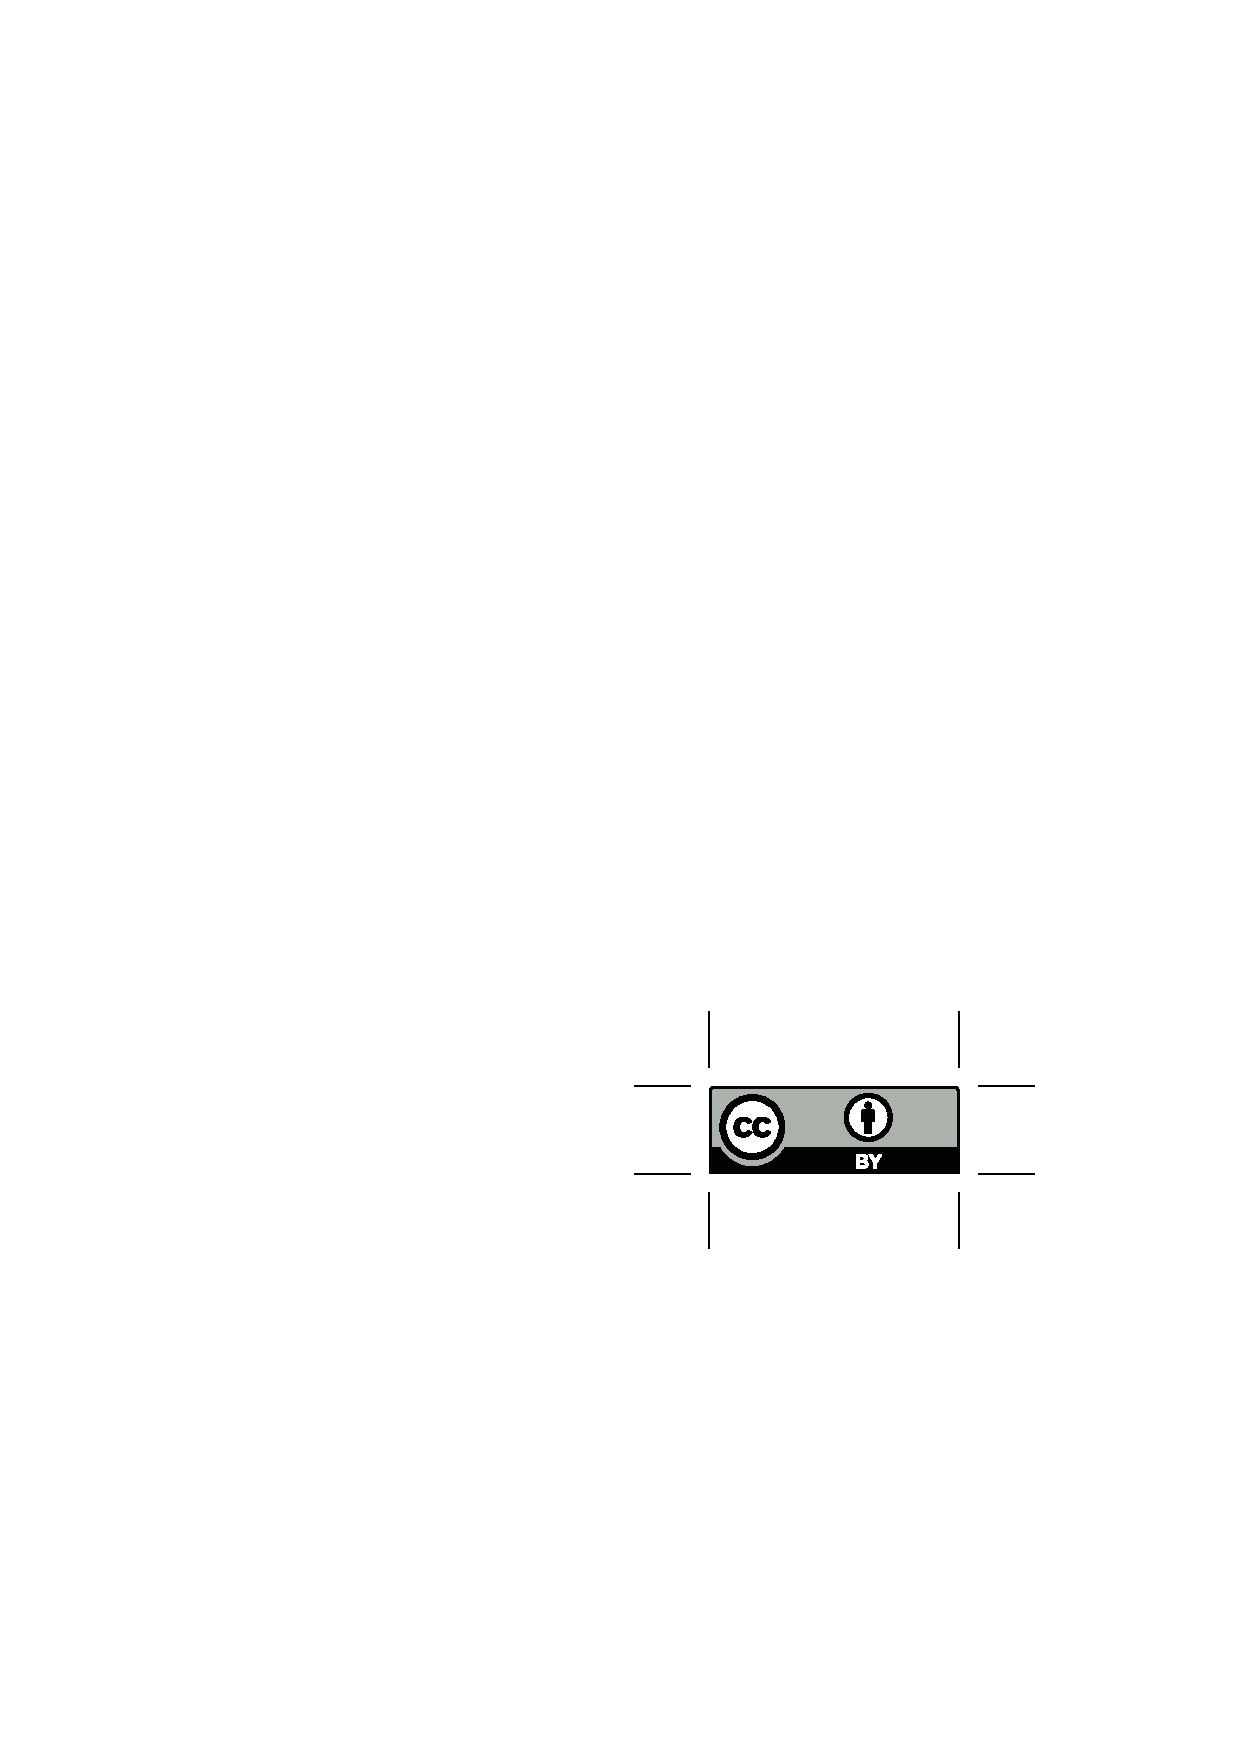
\includegraphics[height=14pt]{by} \\

{\tiny
This work is licensed under a
\href{http://creativecommons.org/licenses/by/4.0/}{Creative Commons Attribution 4.0 International License}.
}}

\begin{document}

\begin{frame}
  \titlepage
\end{frame}

\begin{frame} \frametitle{Big Idea: Randomization}

\emph{Big idea:} a \emph{randomized} algorithm deliberately makes random choices
\begin{itemize}
  \item con: behavior and/or performance becomes \emph{stochastic} (unpredictable)
  \item pro: other aspects can get better (speed, simplicity)
  \item often algorithm gets faster/simpler but analysis gets harder
  \item (this is a win)
\end{itemize}
\vspace{12pt}

\emph A \emph{deterministic algorithm} is not randomized.
\end{frame}

\begin{frame} \frametitle{Recap: Quicksort}
  Recall:
    \begin{itemize}
    \item every sorting algorithm takes $\Omega(n \log n)$ time
    \item merge sort takes $\Theta(n \log n)$ worst-case time and $\Theta(n)$
      space
    \item \textbf{quicksort synopsis:}
    \begin{itemize}
      \item recursive divide-and-conquer
      \item pick random pivot $p$
      \item rearrange list into two zones: $\leq p$ and $> p$
      \item recurse onto each zone
    \end{itemize}
    \item quicksort
    \begin{itemize}
      \item is randomized
      \item $\Theta(n \log n)$ expected time
      \item $\Theta(n^2)$ worst-case time
      \item $\Theta(\log n)$ space
    \end{itemize}
  \end{itemize}
\end{frame}
  
\begin{frame} \frametitle{Recap: Analyzing Randomized Algorithms}
  For each randomized algorithm we make two separate efficiency claims:
  \begin{enumerate}
    \item expected time: the focus
    \item worst-case time: disclaimer; secondary consideration
  \end{enumerate}
  \vspace{12pt}

  ``Quicksort takes $\Theta(n \log n)$ expected time and $\Theta(n^2)$ worst-case time.''
\end{frame}

\begin{frame} \frametitle{Definition of Expected Time}
  Definition: 
  \[ \text{algo.'s expected time} = E[\text{algo.'s worst-case time}] \]

  For random variable $X$ with outcomes $x_1, \ldots, x_n$ of probability $p_1, \ldots, p_n$,
  \[ E[X] = \sum_{\text{outcome $x_i$}} p_i x_i \]

  So
  \[ \text{algo.'s expected time} = \sum_{\text{sequence of random choices $i$}} p_i \cdot (\text{worst-case time steps given } i) \]

\end{frame}

\begin{frame} \frametitle{The Hiring Problem}
  {\footnotesize
  \begin{algorithmic}[1]
    \Function{DETERMINISTIC-HIRE-ASSISTANT}{$A$}
    \State best $ = $ NIL
    \For { $x$ in $A$ }
      \If { best is still NIL or $x$ is better than best }
        \State best $= x$
      \EndIf
    \EndFor
    \State \Return { best }
    \EndFunction
  \end{algorithmic}
  }
  \vspace{24pt}

  Analyze the number of \textbf{reassignments} (line 5)
\end{frame}

\begin{frame} \frametitle{Adversarial Analysis}
  \textbf{Adversarial analysis:} Proof strategy for worst-case analysis
  \vspace{12pt}

  ``Adversary''
  \begin{itemize}
    \item is a fictional opponent character
    \item seeks to show algorithm is inefficient
    \item has full knowledge of algorithm pseudocode
    \item picks least-flattering input
  \end{itemize}
  \vspace{12pt}

  \emph{Big idea:}
  \begin{itemize}
    \item randomization makes the adversary's job harder
    \item so improves the algorithm's expected performance
  \end{itemize}
\end{frame}

\begin{frame} \frametitle{Adversarial Analysis of Deterministic Hiring}
  {\footnotesize
  \begin{algorithmic}[1]
    \Function{DETERMINISTIC-HIRE-ASSISTANT}{$A$}
    \State best $ = $ NIL
    \For { $x$ in $A$ }
      \If { best is still NIL or $x$ is better than best }
        \State best $= x$
      \EndIf
    \EndFor
    \State \Return { best }
    \EndFunction
  \end{algorithmic}
  }
  \vspace{12pt}

  Q: How can an adversary arrange $A$ to maximize reassignments?
  \vspace{12pt}

  Q: What is the worst-case number of reassignments?
\end{frame}

\begin{frame} \frametitle{Randomized Hiring}
  {\footnotesize
  \begin{algorithmic}[1]
    \Function{RANDOMIZED-HIRE-ASSISTANT}{$A$}
    \State Randomly permute $A$ \Comment{ only change }
    \State best $ = $ NIL
    \For { $x$ in $A$ }
      \If { best is still NIL or $x$ is better than best }
        \State best $= x$
      \EndIf
    \EndFor
    \State \Return { best }
    \EndFunction
  \end{algorithmic}
  }
  \vspace{12pt}

  Observe
  \begin{itemize}
    \item the same worst-case scenario exists
    \item \textbf{but}, the adversary cannot force it to occur
  \end{itemize}
\end{frame}

\begin{frame} \frametitle{Randomized Hiring Analysis}
Define
\[ X_i = \{\text{1 if best is reassigned in iteration } i, 0 \text{ otherwise} \} .\]
Observe
\[ X_i = 1 \text{ when the } i\text{th element is the maximum so far} \]
and since $A$ is permuted randomly,
\[ Pr\{X_i=1\} = 1/i \text{ so } E[X_i] = 1/i, \]
and the total number of reassigns is
\[ X = 1/1 + 1/2 + 1/3 + 1/4 + \ldots + 1/n \in O(\log n). \]

\# reassignments is $O(\log n)$ expected and $\Theta(n)$ worst-case.
\end{frame}

%\begin{frame} \frametitle{Birthday Paradox}
%Q: if there are $n$ days in the year, what is the minimum size $k$ of a group of people
%that makes $Pr\{ \text{two people have the same birthday} \} \geq 1/2$? \\
%Intuition: for a given person, each of $n$ days is equally likely, so need $k \geq n/2$
%\end{frame}

\begin{frame} \frametitle{Randomization Patterns}
\emph{Randomization pattern:} approach for using randomization, along with
analysis
\vspace{1cm}

\textbf{Best from random order pattern}: best only gets reassigned expected $O(\log n)$ times,
worst case $\Theta(n)$ times

\end{frame}

\begin{frame} \frametitle{Balls and Bins}
  \begin{center}
    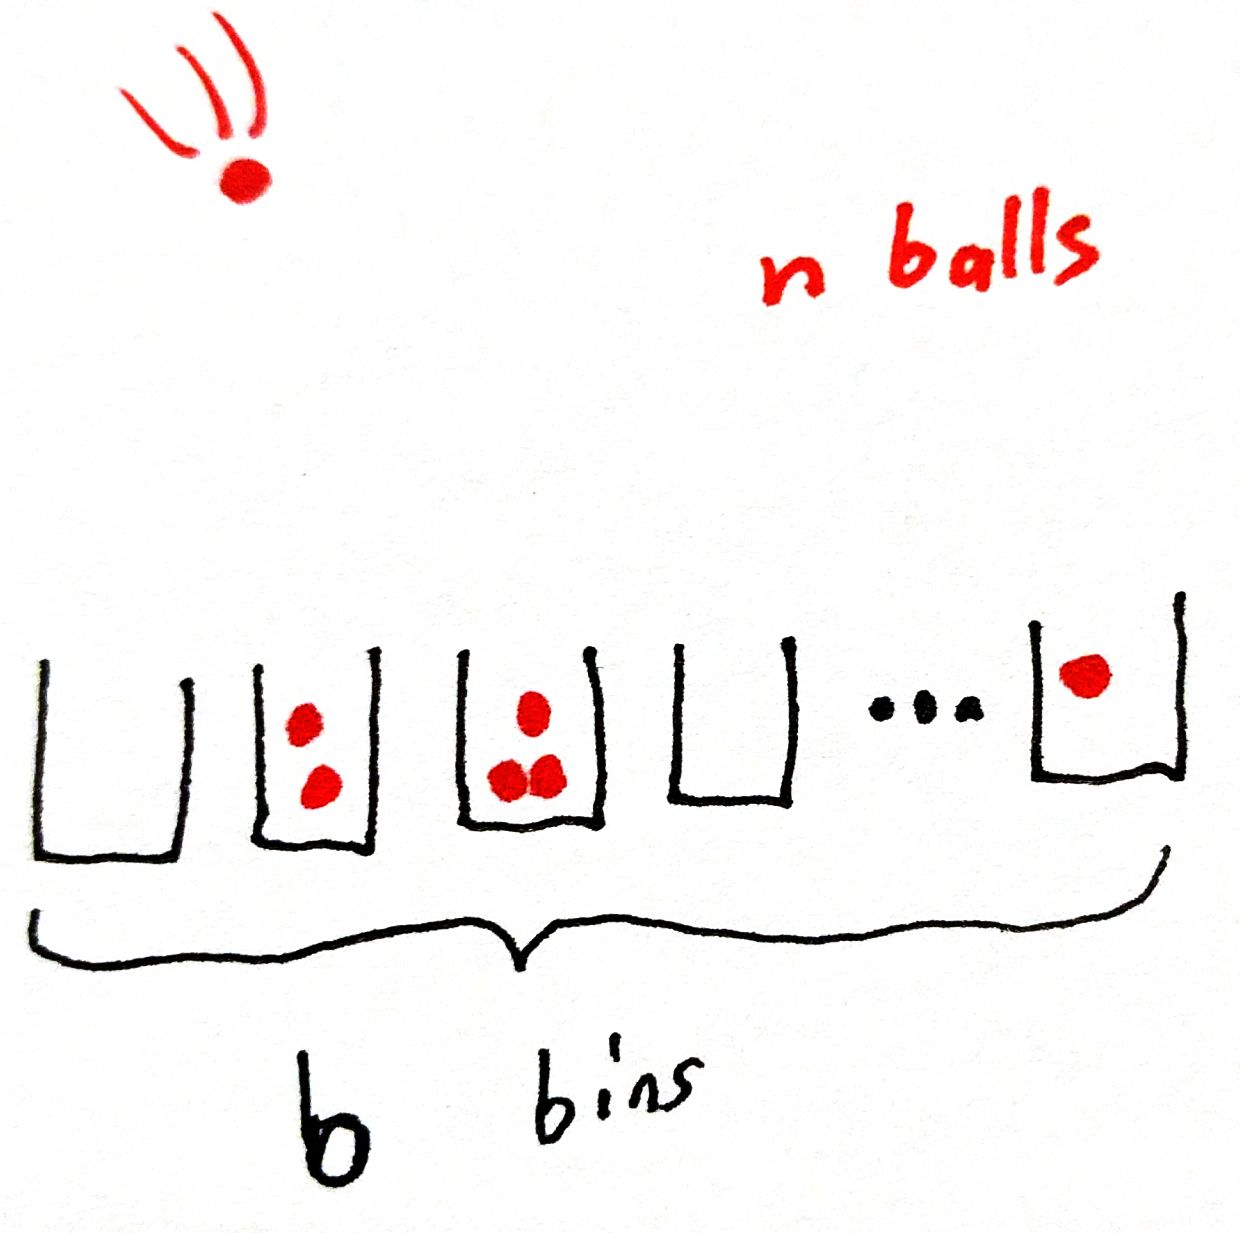
\includegraphics[height=1.5in]{balls-bins.jpg}
  \end{center}

Story to help think about probabilities:
\begin{itemize}
  \item $b$ bins that can hold balls
  \item throw $n$ balls
  \item a ball is equally likely to fall into each bin
  \item corresponds to a game called \emph{plinko}
\end{itemize}
\end{frame}

\begin{frame} \frametitle{Balls and Bins Q \& A}
Answers to questions:
\begin{itemize}
  \item \emph{Q: After $n$ throws, how many balls does a given bin have?} expected $n/b$
  \item \emph{Q: How many throws before a given bin has a ball?} expected $b$
  \item \emph{Q: How many throws before every bin has a ball?} expected $b \ln b \in \Theta(b \log b)$
\end{itemize}
\end{frame}

\begin{frame} \frametitle{Application: Web Server Load Balancer}
  \begin{itemize}
    \item scenario: we have $b$ webservers, $n$ requests coming in, need to route
      each request to one of the servers $1, \ldots, b$
    \item adversary could make expensive requests, so if we take turns in a deterministic
      way, we are vulnerable to a denial-of-service attack
      \begin{itemize}
        \item example: round-robin
      \end{itemize}
    \item So route requests randomly somehow
    \item Idea: choose a \textbf{random} server in $\{1, \ldots, b\}$
    \item Worst-case user experience depends on the heaviest-loaded server
  \end{itemize}
\end{frame}

\begin{frame} \frametitle{With High Probability (WHP)}

\textbf{Terminology:} Let $p(n)$ be the probability that event $X$ occurs as a function of $n;$
then $X$ occurs \emph{with high probability (w.h.p. or WHP)} when
\[ \lim_{n \rightarrow \infty} p(n) = 1. \]

Examples of $p(n)$ bounds considered w.h.p.: $O(1-\frac{1}{n})$, $O(1-\frac{1}{n^2})$, $O(1-\frac{1}{n \log n}).$
\vspace{12pt}

Typically, of the form $O(1-\frac{1}{n^k})$ for $k \geq 1.$
\vspace{12pt}

Intuition: for sufficiently large $n,$ event $X$ is practically certain.
\end{frame}

\begin{frame} \frametitle{Analyzing Random Load Balancing}
\begin{itemize}
  \item suppose $n=b$
  \item suppose the \#balls in a bin is its \emph{load}
  \item high load is bad
  \item \emph{After $n$ throws, what is the maximum load?}
    \[ \frac{\log n}{\log \log n} + o(1) \text{ w.h.p. } \]
  \item Note that for $n \geq 2,$
    \[ \frac{\log n}{\log \log n} \ll \log n . \]
\end{itemize}
\end{frame}

\begin{frame} \frametitle{The Power of Two Random Choices}
\begin{itemize}
  \item \textbf{two random choices}: pick two bins at random, put the ball in
    \emph{the less-loaded bin;} maximum load becomes
    \[ \frac{\log \log n}{\log 2} + \Theta(1) \text{ w.h.p. } \]
  \item Note that $\frac{\log \log n}{\log 2} \ll \frac{\log n}{\log \log n}$; the choosing dramatically decreases maximum load
  \item Intuition: what random events lead to a high load in each scenario?
  \item generally, if we make \textbf{$d$ random choices}, maximum load is
    \[ \frac{\log \log n}{\log d} + \Theta(1) \text { w.h.p. } \]
  \item very slow-growing, nearly constant
\end{itemize}
\end{frame}

\begin{frame} \frametitle{Load Balancing Patterns}

\textbf{Balance load with one random choice}: for $n$ balls in $\Theta(n)$ bins,
expected load is $\Theta(1)$ and maximum load is $\Theta(\frac{\log n}{\log \log n})$ w.h.p.
\vspace{.5cm}

\textbf{Balance load with $d$ random choices}: expected load is still $\Theta(1),$
and maximum load is $\Theta(\frac{\log \log n}{\log d})$ w.h.p.
\vspace{.5cm}

Trade-off:
\begin{itemize}
  \item one random choice: choosing bin involves only one random number,
  $\Theta(1)$ time, and
    does not involve state of bins; \emph{but} load can be more uneven
  \item $d$ random choices: choosing bin involves querying the state of $\Theta(d)$ servers, but
  load is distributed \textbf{extremely} evenly
\end{itemize}
\end{frame}

\begin{frame} \frametitle{Streaks}
\begin{itemize}
  \item suppose we flip a fair coin, so $Pr\{\text{heads}\} = Pr\{\text{tails}\}=\frac{1}{2}$
  \item \emph{streak:} sequence of the same result (seq. of heads, or seq. of tails)
  \item \emph{Q: After $n$ flips, what is the longest streak?}
  \item A: expected length of the longest streak is $\Theta(\log n)$
\end{itemize}
\end{frame}

\begin{frame} \frametitle{Hash Tables}
Review hash tables
\begin{itemize}
  \item can store a \textbf{set} of \emph{keys}
  \item or a \textbf{map} from keys to arbitrary \emph{values}
  \item keys must \emph{hashable:} either integers, or can be mapped deterministically
    to integers (e.g. strings, floats, tuples of hashable objects, etc.)
  \item a search, insert, or delete operation takes $\Theta(1)$ expected time and
    $\Theta(n)$ worst-case time
  \item many variants with trade-offs: chaining vs. open addressing, universal vs.
    tabular functions, cuckoo, robin hood, etc.
\end{itemize}
\end{frame}

\begin{frame} \frametitle{Hash Set Operations}
  \begin{center}
    \begin{tabular}{llll}
      \textbf{Operation} & \textbf{Pseudocode Example} & \textbf{Exp. Time} & \textbf{W.C. Time} \\ \hline
      Create empty hash set & \texttt{S = HashSet()} & $\Theta(1)$ & $\Theta(1)$ \\
      Insert an element & \texttt{S.insert(x)} & $\Theta(1)$ & $\Theta(n)$ \\
      Remove an element & \texttt{S.remove(x)} & $\Theta(1)$ & $\Theta(n)$ \\
      Search for an element & \texttt{if S.contains(x):} & $\Theta(1)$ & $\Theta(n)$ \\
    \end{tabular}
  \end{center}

  \vspace{12pt}
  Recall: A math set cannot have duplicates, so inserting the same $x$ multiple times leaves only one copy in the set.
\end{frame}

\begin{frame} \frametitle{Hash Map Operations}
  \begin{center}
    \begin{tabular}{llll}
      \textbf{Operation} & \textbf{Pseudocode Example} & \textbf{Exp. Time} & \textbf{W.C. Time} \\ \hline
      Create empty hash map & \texttt{M = HashMap()} & $\Theta(1)$ & $\Theta(1)$ \\
      Insert $k, v$ & \texttt{M.insert(k, v)} & $\Theta(1)$ & $\Theta(n)$ \\
      Remove key $k$ & \texttt{S.remove(k)} & $\Theta(1)$ & $\Theta(n)$ \\
      Search for key $k$ & \texttt{if S.contains(k):} & $\Theta(1)$ & $\Theta(n)$ \\
      Lookup key $k$ & \texttt{S.get(k)} & $\Theta(1)$ & $\Theta(n)$ \\
    \end{tabular}
  \end{center}

  \vspace{12pt}
  Recall: Each key must be distinct, so re-inserting a new value for key $k$ overwrites the old value.
\end{frame}

\begin{frame} \frametitle{Reduce-to-Hash-Tables Pattern}
\begin{itemize}
  \item make critical use of a hash set or hash map
  \item replace a $\Theta(n)$ loop with a $\Theta(1)$ expected-time hash table operation
  \item good: fast, simple
  \item bad: time efficiency becomes \emph{expected}
\end{itemize}
\end{frame}

\begin{frame} \frametitle{Duplicate Removal Problem}
  \emph{duplicate removal problem} \\
  \textbf{input:} an array $A[1..n]$ of objects\\
  \textbf{output:} a list $D$ of the distinct elements of $A$ (i.e. duplicates
    are removed)\\

\end{frame}

\begin{frame} \frametitle{Duplicate Removal -- Baseline Pseudocode}
  {\footnotesize
  \begin{algorithmic}[1]
    \Function{REMOVE-DUPLICATES-BASELINE}{$A$}
    \State $D$ = new list
    \For { $a$ in $A$ }
        \State already-present $ = $ False
        \For { $d$ in $D$ }
          \If { $a$ == $d$ }
            \State already-present $ = $ True
          \EndIf
        \EndFor
        \If { not already-present }
          \State $D$.add($a$)
        \EndIf
    \EndFor
    \State \Return { $D$ }
    \EndFunction
  \end{algorithmic}
  }
\end{frame}

\begin{frame} \frametitle{Duplicate Removal -- Baseline Analysis}
  \begin{itemize}
    \item outer loop: $n$ iterations
    \item inner loop: $\Theta(n)$ time
    \item total $\Theta(n^2)$ time
    \item bottleneck is the nested loops
    \item \emph{Reduce-to-Hash-Tables Pattern:} replace the inner loop with a hash table operation
  \end{itemize}
\end{frame}

\begin{frame} \frametitle{Duplicate Removal -- Improved Algorithm}
  {\footnotesize
  \begin{algorithmic}[1]
    \Function{REMOVE-DUPLICATES-RANDOMIZED}{$A$}
    \State $HS$ = HashSet()
    \For { $x$ in $A$ }
      \If { not $HS$.contains($x$) }
        \State $HS$.insert($x$)
      \EndIf
    \EndFor
    \State $D = $ insert each element of $HS$ into a list \Comment{ match \textbf{output:} data type }
    \State \Return { $D$ }
    \EndFunction
  \end{algorithmic}
  }
  \vspace{.3cm}
  $\Theta(n)$ expected time, $\Theta(n^2)$ worst-case time.
\end{frame}

\begin{frame} \frametitle{Duplicate Removal -- Analyze Trade-Offs}
  \begin{itemize}
    \item baseline: $\Theta(n^2)$ time; more complicated; not dependent on hash tables knowledge
    \item randomized: $\Theta(n)$ expected time, $\Theta(n^2)$ worst-case time; simpler; depends on hash tables
    \item randomized is superior
    \item pay-off for learning about data structures!
  \end{itemize}
\end{frame}

\begin{frame} \frametitle{Planning a Hash Set}
\begin{itemize}
  \item hash set stores \emph{key-value} associations
  \item each key is linked to a value
  \item \emph{key:} identity of a thing
  \item \emph{value:} information associated with that thing
  \item insert, remove, search
  \item Strategy: fill in the blanks ``Given \_\_\emph{key}\_\_, update \_\_\emph{value}\_\_ .''
  \item Strategy: write out concrete data in a table like
  \begin{center}
    \begin{tabular}{ll}
      \textbf{Key} & \textbf{Value} \\ \hline
      key 1 & value 1 \\
      key 2 & value 2 \\
      $\ldots$ & $\ldots$ 
    \end{tabular}
  \end{center}
\end{itemize}
\end{frame}


\begin{frame} \frametitle{Mode Problem}
  \emph{duplicate removal problem} \\
  \textbf{input:} a list $A$ of $n$ elements\\
  \textbf{output:} a most-frequently-ocurring element of $A$ \\

  \vspace{24pt}
  Note:
  \begin{itemize}
    \item $A$ is a list, not a set, so $A$ may have duplicates
    \item in the event of ties, any of the ties may be output
  \end{itemize}
\end{frame}


\begin{frame} \frametitle{Mode -- Baseline Pseudocode}
  {\footnotesize
  \begin{algorithmic}[1]
    \Function{MODE-BASELINE}{$A$}
    \State mode = NIL
    \State mode-count = 0
    \For { $a$ in $A$ }
      \State a-count = 0
      \For { $b$ in $A$ }
        \If { $b$ == $a$ }
          \State a-count++
        \EndIf
      \EndFor
      \If { a-count $>$ mode-count }
        \State mode = $a$
        \State mode-count = a-count
      \EndIf
    \EndFor
    \State \Return {mode}
    \EndFunction
  \end{algorithmic}
  }
\end{frame}

\begin{frame} \frametitle{Mode -- Baseline Analysis}
  \begin{itemize}
    \item total $\Theta(n^2)$ time
    \item again, bottleneck is the nested loops
    \item \emph{Reduce-to-Hash-Tables Pattern:} replace the inner loop with a hash table operation
    \item Pre-compute each element's count
    \item Hash map:  ``Given (an element), update (its count) .''
    \item Concrete data :
    \[A = \langle 3, 1, 7, 1, 1, 1, 7 \rangle \]
    \begin{center}
      \begin{tabular}{ll}
        \textbf{Key} & \textbf{Value} \\ \hline
        3 & 1 \\
        1 & 4 \\
        7 & 2 \\
      \end{tabular}
    \end{center}
  \end{itemize}
\end{frame}


\begin{frame} \frametitle{Mode -- Second Draft}
  Hash table is used to speed up first draft, but we haven't initialized it yet.
  \vspace{12pt}

  {\footnotesize
  \begin{algorithmic}[1]
    \Function{MODE-RANDOMIZED}{$A$}
    \State \emph{(somehow create and populate hash map ElementToCount)}
    \State mode = $A[0]$
    \State mode-count = 0
    \For { $a$ in $A$ }
        \State a-count = ElementToCount.get($a$)
        \If { a-count $>$ mode-count }
          \State mode = $a$
          \State mode-count = a-count
      \EndIf
    \EndFor
    \State \Return {mode}
    \EndFunction
  \end{algorithmic}
  }
\end{frame}


\begin{frame} \frametitle{Mode -- Final Draft}
  {\footnotesize
  \begin{algorithmic}[1]
    \Function{MODE-RANDOMIZED}{$A$}
    \State ElementToCount = HashMap()
    \For { $a$ in $A$ }
      \If{ ElementToCount.contains($a$) }
        \State ElementToCount.set($a$, ElementToCount.get($a$) $+ 1$)
      \Else
        \State ElementToCount.set($a$, 1)
      \EndIf
    \EndFor
    \State mode = $A[0]$
    \State mode-count = 0
    \For { $a$ in $A$ }
        \State a-count = ElementToCount.get($a$)
        \If { a-count $>$ mode-count }
          \State mode = $a$
          \State mode-count = a-count
      \EndIf
    \EndFor
    \State \Return {mode}
    \EndFunction
  \end{algorithmic}
  }
\end{frame}


\begin{frame} \frametitle{Duplicate Removal -- Analyze Trade-Offs}
  \begin{itemize}
    \item baseline: $\Theta(n^2)$ time
    \item randomized:
      \begin{itemize}
        \item first loop: $\Theta(n)$ expected, $\Theta(n^2)$ worst-case
        \item second loop: same
        \item everything else: $\Theta(1)$
        \item total: $\Theta(n)$ expected, $\Theta(n^2)$ worst-case
        \item like the maximum subarray algorithm, refactoring two nested loops into two sequential loops speeds things up
      \end{itemize}
    \item again, randomized is superior
  \end{itemize}
\end{frame}

\end{document}
